\documentclass[a4paper]{article} %\documentclass[]{article}
\usepackage[utf8]{inputenc}
\usepackage{graphicx}
\usepackage{float} % H positioning
\usepackage{lscape}

\usepackage{listings}

\usepackage [english]{babel}
\usepackage [autostyle, english = american]{csquotes}

% head and footer
\usepackage{fancyhdr}
\pagestyle{fancy}
\fancyhf{}
\fancyhead[LE,RO]{\thepage}
\fancyhead[RE,LO]{\leftmark}
%\fancyfoot[CE,CO]{\leftmark}
%\fancyfoot[LE,RO]{\thepage}
\fancyfoot[LE,RO]{\thepage}
\fancyfoot[RE,LO]{\rightmark}
\renewcommand{\headrulewidth}{2pt}
\renewcommand{\footrulewidth}{1pt}


%code
\usepackage{lmodern}  % for bold teletype font
\usepackage{amsmath}  % for \hookrightarrow
\usepackage{amssymb} % for math symbols
\usepackage{xcolor}   % for \textcolor

\usepackage{booktabs} % for tables https://people.inf.ethz.ch/markusp/teaching/guides/guide-tables.pdf
\newcommand{\ra}[1]{\renewcommand{\arraystretch}{#1}}


\definecolor{eclipseStrings}{RGB}{42,0.0,255}
\definecolor{eclipseKeywords}{RGB}{127,0,85}
\colorlet{numb}{magenta!60!black}
\lstdefinelanguage{json}{
	basicstyle=\normalfont\ttfamily,
	commentstyle=\color{eclipseStrings}, % style of comment
	stringstyle=\color{eclipseKeywords}, % style of strings
	numbers=left,
	numberstyle=\scriptsize,
	stepnumber=1,
	numbersep=8pt,
	showstringspaces=false,
	breaklines=true,
	frame=lines
	string=[s]{"}{"},
	comment=[l]{:\ "},
	morecomment=[l]{:"},
	literate=
	*{0}{{{\color{numb}0}}}{1}
	{1}{{{\color{numb}1}}}{1}
	{2}{{{\color{numb}2}}}{1}
	{3}{{{\color{numb}3}}}{1}
	{4}{{{\color{numb}4}}}{1}
	{5}{{{\color{numb}5}}}{1}
	{6}{{{\color{numb}6}}}{1}
	{7}{{{\color{numb}7}}}{1}
	{8}{{{\color{numb}8}}}{1}
	{9}{{{\color{numb}9}}}{1}
}

\usepackage[hidelinks]{hyperref}


\begin{document}
	
	%opening
	\begin{titlepage}
		\centering
		\vspace*{1cm}
		%\includegraphics[width=0.20\textwidth]{images/logo_unipd.png}\par\vspace{1cm}
		{\par \scshape\LARGE Università degli Studi di Padova \par}
		\vspace{1cm}
		{\scshape\Large Dipartimento di Ingegneria dell'Informazione\\Corso di Laurea Magistrale in Ingegneria Informatica\par}
		\vspace{1.5cm}
		{\huge\bfseries Online contextual system tuning with Bayesian Optimization and Workload Forecasting\par}
		\vspace{2cm}
		{ \large \itshape Laureando:}
		{ \large Luca \textsc{Moroldo} \par}
		\vspace{0.7cm}
		{ \large \itshape Relatore:}
		{ \large Prof. Nicola \textsc{Ferro} \par}
		\vfill
		
		% Bottom of the page
		{ \large 25 Settembre 2019 \par}
		{ \large \textsc{Anno Accademico 2018/2019}\par}
	\end{titlepage}
	
	% empty page
	\clearpage%
	\thispagestyle{empty}%
	\addtocounter{page}{-1}%
	\null%
	\clearpage
	
	\newpage
	\pagenumbering{roman}
	\thispagestyle{plain}
	\section*{Sommario}
	
	Summary here
	
	
	% empty page
	\clearpage%
	\thispagestyle{empty}%
	\addtocounter{page}{-1}%
	\null%
	\clearpage
	
	% Custom TOC title
	\renewcommand{\contentsname}{Indice}
	\newpage
	\thispagestyle{plain}
	\tableofcontents

	% empty page
	\clearpage%
	\thispagestyle{empty}%
	\addtocounter{page}{-1}%
	\null%
	\clearpage
	
	
	% =================== INTRODUZIONE ==========================
	
	\newpage
	\pagenumbering{arabic}
	
	\section{ Introduction }
	Add context and motivation: we are optimizing IT systems and we want to do that online, using the real workload, which requires bla bla presented in section state of the art.
	
	\section{ Context and State of the Art }
	In order to apply Contextual Bayesian Optimization (BO) to automatically tune IT systems in an online manner, where the system is receiving the production workload, two key components are required: a workload characterization and a workload forecasting module. \\
	This section first briefly presents BO explaining why workload characterization is required. Then, the state of the art of forecasting will be presented, followed by a section on workload forecasting in the context of IT systems. 
	
	\subsection{ Bayesian Optimization }
	Bayesian Optimization \cite{BO} is a tool for the joint optimization of design choices of complex systems, such as the parameters of a recommendation system, a neural network, or a medical analysis tool. For example a typical software system made of a database, a back-end, and a front-end is characterized by an enormous amount of parameters that are often dependent on each other.
	Optimizing such parameters is not a simple task, and BO provides an automated approach to make such design choices.\\
	
	Mathematically, the goal is to maximize (or minimize) an unknown objective function $f$:\\
	\begin{equation} \label{eq:bo_optimization}
				\pmb{x}^\star = \underset{\pmb{x} \in \mathcal{X}}{\mathrm{argmax}} f(\pmb{x})
	\end{equation}
	where $\mathcal{X}$ is the design space of interest, e.g. a compact subset of $\mathbb{R}^d$. In general, $f$ can be any black-box function with no simple closed form function that can be evaluated at any arbitrary point in the domain $\mathcal{X}$, where the evaluation can produce noise-corrupted outputs $y \in \mathbb{R}$.\\
	BO is a sequential approach to solve equation \ref{eq:bo_optimization}: at every iteration $i$, the algorithm selects a new $\pmb{x}_{i+1}$ at which $f$ is queried, resulting in a measurement $y_i$. When the maximum number of iterations is reached, or when $y^\star$ is a satisfactory outcome, the algorithm stops returning the best configuration $\pmb{x}^\star$ associated with the best outcome $y^\star$. BO is very data efficient, making it useful when the evaluations of $f$ are costly: the model is initialized with a prior belief, and then at each iteration it is refined using observed data via Bayesian posterior updating. The acquisition function $\alpha_n : \mathcal{X} \rightarrow \mathbb{R}$ guides exploration by evaluating candidate points in $\mathcal{X}$, meaning that $\pmb{x}_{i+1}$ is selected by maximizing $\alpha_n$ using data up to iteration $i$. Figure \ref{fig:bo} shows a few iterations of BO.
	\begin{figure} \label{fig:bo}
		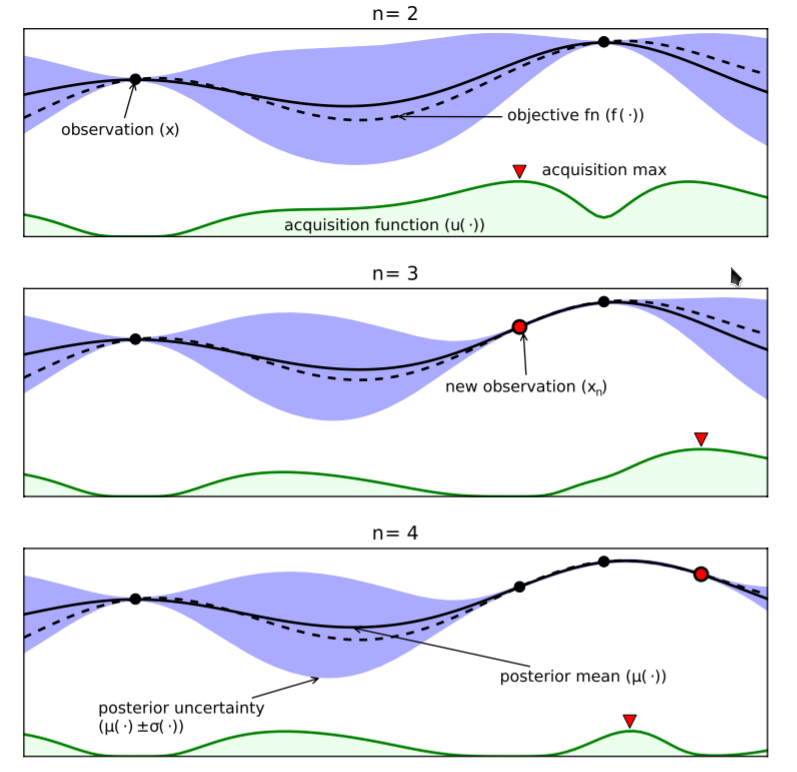
\includegraphics[width=\linewidth]{img/bo.png}
		\caption{A few iterations of BO. The acquisition function in green guides the selection of the next point, obtaining a new observation $(\pmb{x}_i, y_i)$} that updates the underlying model.
	\end{figure}
	The acquisition function $\alpha_n$ provides a trade off between exploration and exploitation: when boosting exploration the value of $\alpha_n$ will be higher in areas of uncertainty, while when boosting exploitation $\alpha_n$ will favor locations where the surrogate model predicts a high objective. It is critical for the acquisition function to be cheap to evaluate or approximate, especially in relation to the objective function $f$.
	
	In summary, BO has two key ingredients \cite{BO}: a probabilistic surrogate model, consisting of a prior distribution that captures our beliefs about $f$ and an observation model that describes the data generation process, and a loss function that describes how optimal a sequence of queries are. The expected loss is minimized to drive the selection of $\pmb{x}_i$. After observing the outcome $y_i$ of $\pmb{x}_i$, the prior is updated to produce a more informative posterior distribution.
	
	Finally, when dealing with a family of correlated objective functions $\mathcal{T}=\{f_1, ..., f_m\}$, such as the performance of an IT system under different workloads or the same IT system running with different software versions, it may be useful to use data obtained optimizing $f_i$ to optimize $f_j$. BO has been extended to deal with such multitask scenario by sharing information between the black-box functions in $\mathcal{T}$: figure \ref{fig:multitask_bo} shows how data from two functions (green and red) influences the posterior predictive distribution of the blue function.
	\begin{figure} \label{fig:multitask_bo}
		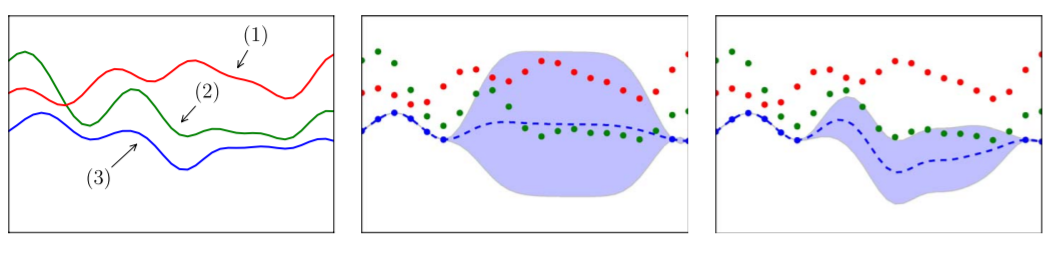
\includegraphics[width=\linewidth]{img/multitask_bo.png}
		\caption{Multitask Bayesian Optimization.}
	\end{figure}
	
	\subsubsection{Contextual Bayesian Optimization of IT systems} \label{ssec:contextual_bayesian_optimization}
	
	When applying BO to IT systems, the goal is to find a configuration $\pmb{x}$ to optimize a performance indicator $y \in \mathbb{R}$ such as throughput, response time, and memory consumption \cite{AkamasCGP}. If BO is applied while the system is running, it is very likely that the workload will change over time: the number of users connected to the system can increase and decrease, as their behavior can change from read-intensive to write-intensive operations. Such changes will inevitably affect how the system behaves under a specific configuration, but regardless the workload the underlying system maintains some properties. This scenario fits perfectly the contextual extension of BO \cite{CGPBanditOptimization}.
	
	More formally, we are trying to maximize a function $f_{\pmb{w}}$ subject to a workload $\pmb{w}_t$ that changes over time. The tuning process, shown in figure \ref{fig:cgp_it_sys}, starts with a configuration $\pmb{x}_0$ (usually the default configuration, called baseline) applied under a workload $\pmb{w}_0$ whose performance indicator $y_0$ is measured. The tuner uses a knowledge base, initially containing only the triplet $\{(\pmb{x}_0, \pmb{w}_0, y_0)\}$, along with the current workload $w_1$ to suggest a new configuration $x_1$ that is applied, evaluated, and added to the knowledge base. After $N$ iterations the tuner can exploit all information $(\{(\pmb{x}_0, \pmb{w}_0, y_0)\}, ..., \{(\pmb{x}_N, \pmb{w}_N, y_N)\})$ gathered so far to make refined suggestions.
	\begin{figure} \label{fig:cgp_it_sys}
		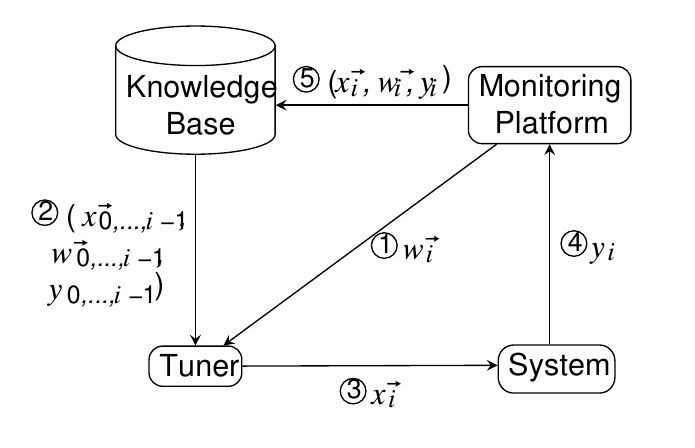
\includegraphics[width=\linewidth]{img/cgp_it_sys.png}
		\caption{Tuning process - TODO disallineata}
	\end{figure}
	Furthermore, when optimizing a system, it may be useful to define some constraints the system should not violate: a tuning process may be executed with the requirement satisfying some Quality of Service (QoS) levels. For example, while trying to minimize the average CPU usage to reduce the infrastructure costs, the system could be expected to keep the users' requests latency below some target.  The work proposed by \cite{AkamasCGP} has been extended so that it is possible to define such constraints: when a configuration violates any constraint, the violation is added to the knowledge base along along with its configuration and associated system performance. Interestingly, the tuner could be used on a system that doesn't initially satisfy some QoS levels, so that at the end of the tuning process violations are not likely to occur anymore.
	
	The BO regression model is a Gaussian Process (GP) which derives its posterior model (i.e. the predictions) by combining observed values with its prior distribution. To make GP able to explore uncertain regions, i.e. configurations that are different from the ones in the knowledge base, it should not resort to its prior distribution \cite{AkamasCGP} so that unknown configurations are not predicted to ruin the performance of the IT system. To do so, the observed data is standardized and GP will predict that by picking a random configuration the system will exhibit a performance value that is equal to the average performance of the observed values. Nonetheless, when dealing with different workloads, it is crucial to standardize each point by taking into account the relevant workload \cite{AkamasCGP}. This can be achieved by using a modified version of the Normalized Performance Improvement:\\\\
	\centerline{
	$
	NPI(\pmb{x}, \pmb{w}) = \frac{f(\pmb{x}_0, \pmb{w}) - f(\pmb{x}, \pmb{w})}{f(\pmb{x}_0, \pmb{w}) - f(\pmb{x}^+_{\pmb{w}}, \pmb{w})}
	$
	}\\\\
	where $\pmb{x}$ is the configuration being evaluated, $\pmb{x}_0$ is the baseline configuration, $\pmb{w}$ is the workload, and $f(\pmb{x}^+_{\pmb{w}}, \pmb{w})$ is the best configuration found so far while tuning the system with the workload $\pmb{w}$. Hence, \cite{AkamasCGP} requires a workload characterization module to cluster the workloads and effectively apply BO. Workload characterization is discussed in section \ref{ssec:workload_characterization}.
	
	To evaluate the performance of an IT system under a new configuration, many technologies require some warm up time. For example, the Java Virtual Machine is characterized by a lazy class loading and Just In Time (JIT) compilation that make the performance evolve over time after the Java application is launched. Usually, a window of duration that ranges from ten to thirty minutes is required for the performance to stabilize. Furthermore, after the warm up is completed, the system performance $y_i$ resulting from the configuration $\pmb{x}_i$ under workload $\pmb{w}_i$ should be obtained by taking multiple measurements in order to balance the noisy environment. This evaluation process requires the workload to remain stable in order to avoid corrupting the measurements or nullifying the warm up (e.g. a new workload may use different Java classes and functions). Therefore, a single tuning step (or experiment) requires a time window $\omega_{t_1:t_2}$, starting at time $t_1$ and ending at time $t_2$, of duration $t_2 - t_1$ during which the workload $w_t$ must be stable.\\
	Furthermore, as mentioned before, Contextual Bayesian Optimization suggests a configuration tailored for the given workload.  This means that a workload change may cause the system being optimized to under perform, potentially leading to bad QoS or even failures. Such consequences should be avoided as much as possible.
	
	In order to predict if the upcoming tuning window will be stable the tuner requires a component capable of predicting the upcoming workload, as long as some sort of classifier that given the predicted workload indicates whether the future workload will be stable or not.
	Finally, once the performance of the best configuration for the given workload is satisfactory, that configuration can be applied in advance.\\
	Forecasting and workload forecasting will be discusses in section \ref{sec:forecasting} and \ref{ssec:workload_forecasting}	
	
	\subsection{Workload characterization} \label{ssec:workload_characterization}
	% wkld charact è stata usata anche per decidere come fare i processori(MICROARCHITECTURE-INDEPENDENT WORKLOAD CHARACTERIZATION)
	The term workload refers to all the inputs received by a given technological infrastructure \cite{WorkloadCharacterization}. Understanding the properties and behavior of such workload is essential for evaluating the Quality of Service (QoS) perceived by the users in order to meet the Service Level Agreement (SLA) obligations. In such context, workload characterization provides the basis for devising efficient resource provisioning, power management, and performance engineering strategies.\\
	By characterizing the workload and deriving workload models it is possible to summarize and explain the main properties of the workloads, generate synthetic workloads for performance evaluation studies, and define benchmark experiments. Workload characterization can be applied to different domains such as online social networks, video services, mobile devices, and cloud computing.
	
	Characterizing the workloads requires to collect representative measurements while the system under study is operating (i.e. under the true workloads). These measurements refer to specific components of the system and capture their static and dynamic properties, along with the behavior of the users. It is important to take into account the hierarchical nature of the typical infrastructures: a network sniffer provides measurements about the network traffic, logging facilities provide application-specific measurements such as the number of requests to an URL of a web application, and tracelogs contain measurements related to the resources used by jobs and tasks (e.g. CPU and memory usage). The choice of the attributes to consider for the characterization depends on its objectives and on the nature of the workload to be analyzed.
	
	Once measurements are collected, they have to be analyzed in order to build workload models. The first step is to perform a statistical analysis to describe the properties (e.g. mean, variance, percentiles) of each attribute of interest and find any relation between them (e.g. using Pearson's correlation coefficient \cite{PearsonCoefficient}). \\
	A common challenge faced during this step is how to deal with outliers, that are atypical behaviors of one or more attributes: outliers could indicate previously unknown phenomena that are worth exploring, or they could correspond to anomalous operating conditions that should be discarded.
	
	Further steps of the workload characterization methodology are multivariate analysis to analyze the components in the multidimensional space of their attributes, numerical fitting to study the dynamics of the workloads and model their temporal patterns, stochastic processes to study time-varying properties of the workloads, and graph analysis to model the behavior of interactive users \cite{WorkloadCharacterization}.
	
	Multivariate analysis allows to derive models that capture and summarize the overall properties of the workloads. A technique that has been widely used for that purpose is clustering \cite{ClusteringSurvey}, which enables unsupervised classification when labeled data is not available. A popular clustering algorithm is $k$-means \cite{ClusteringSurvey}, that partitions the data into $k$ clusters identified by $k$ centroids where each centroid would represent one type of workload. Clustering is further presented in section \ref{ssec:clustering}.\\
	When the number of variables being analyzed is too large, it is common to apply dimensionality reduction techniques such as PCA \cite{PCA} to obtain a smaller set of uncorrelated variables.
	
	With numerical fitting techniques is possible to estimate the parameters of the function that best fits the empirical data, for example to understand whether it is generated by a well-known probabilistic distribution. \cite{WorkloadsPowerLaw} has shown that the distribution of many workloads properties are well described by power laws (e.g. Pareto or Zipf distributions), meaning that extreme values should be investigated rather than being considered outliers.
	
	Finally, stochastic processes such as wavelets and nonparametric filtering are used to extract trend and seasonal components from the time series representing the workload properties (see section \ref{sec:forecasting}), identify the structure of predictive models and estimate their parameters. A common goal when applying such techniques is to cope with capacity planning and resource management.
	
	\subsection{ Clustering } \label{ssec:clustering}
	aaa
	
	
	\subsection{ Forecasting } \label{sec:forecasting}
	Forecasting is a common data science task that makes use of temporal data \cite{ForecastingSurvey} to help organizations with capacity planning, goal setting, and anomaly detection. It is required in many situations: for example, deciding whether to build another warehouse in the next five years requires forecasts of future demand, and scheduling staff in a call center next week requires forecasts of call volumes.
	
	The first successful forecasting methods have been proposed around \textit{1950}, some of them being Exponential Smoothing \cite{ExponentialSmoothingHoltCharles} and ARIMA \cite{ForecastingBoxJenkins}, which originated a wide variety of derived techniques \cite{25YearsForecasting}. In the big-data era, where companies have huge numbers of time series each with their own characteristics, traditional techniques have shown some limitations due to specific model requirements (section \ref{sssec:exponential_smoothing} and \ref{sssec:arma}), model inflexibility, necessity of manual feature engineering, lack of automation, difficulties of dealing with missing data, and lack of well-performing multivariate models \cite{25YearsForecasting}.\\
	Recent developments have seen pure deep learning models joining the fields with inconsistent performance \cite{DeepLearningForecastingSurvey}, but highlighting the possibility of exploiting huge datasets in order to learn a single global model capable of recognizing complex and sometimes shared time series patterns. Other recent deep learning research achievements, especially in the natural language processing domain \cite{RNNLSTM, seq2seq, EncoderDecoder}, have inspired promising models \cite{DeepAR, DeepState, DeepLearningForecastingSurvey}, some of them having an hybrid architecture that utilizes both statistical and machine learning (ML) features \cite{MAKRIDAKIS2018802, GluonTS}. 
	Interestingly, the winner of the 2018 M4 competition \cite{MAKRIDAKIS2018802} was a combination of Exponential Smoothing and deep learning \cite{UberHybridES}, while the top-performing submissions of the 2020 M5 competition \cite{M5Competition}, where most of the time series have some kind of correlation and share frequency and domain, cross-learning ML models have shown their potential with the top-performing submissions using a weighted average of several pure ML models.\\
	Other methods, such as the one proposed by Prophet \cite{FacebookProphet}, provide an analyst-in-the-loop approach suggesting that by injecting domain-specific knowledge into the model it's still possible to outperform fully automated approaches, especially with small amounts of data.\\
	Nevertheless, Artificial Neural Network (ANN) based models have only recently started overtaking simpler classical models \cite{MAKRIDAKIS2018802, M5Competition} opening a set of inspiring possibilities, and the market has seen big companies developing their own solutions \cite{FacebookProphet, GluonTS, MicrosoftSSA, UberHybridES} highlighting the necessity for the businesses of better forecasting techniques.
	
	Despite the forecasting importance, there are still serious challenges associated with producing reliable and high quality forecasts: time series often have long term dependencies with nonlinear relationships.  Moreover, the quality of forecasts are heavily affected by model selection, model tuning, and covariates (e.g. dynamical historical features) selection, where the data scientist has to manually inspect data and inject domain knowledge into the model \cite{DeepLearningForecastingSurvey, FacebookProphet}.\\
	The necessity of tailored forecasting models comes from the fact that time series can be very different from each other, exhibiting complex patterns and relationships with other time series and data in general. 
	
	Nevertheless, time series can often be seen as a composition of a trend, a seasonal pattern, and a cycle \cite{ForecastingHyndmanAthanasopoulos}.
	A trend exists if there is a long-term increase or decrease in the data, which can be linear or not, and can be subject to changes that increase or decrease the trend.
	A seasonal pattern occurs when a time series is affected by seasonal factors like the hour of the day or the day of the week, with fixed and known frequency.
	Finally, a cycle occurs when data rises and falls without a fixed frequency, e.g. due to economic conditions.  Cycles are usually longer than seasonal patterns and have more variable magnitudes.
	
	\begin{figure}
	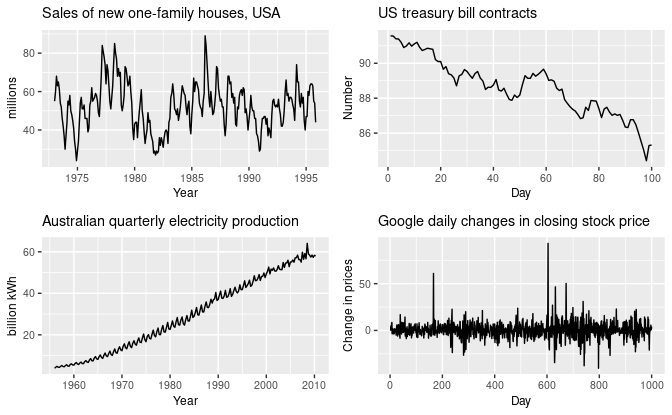
\includegraphics[width=\linewidth]{img/sota_ts_components.png}
	\caption{Four time series examples. Top left: seasonality and cycle; top right: trend only; bottom left: trend and seasonality; bottom right: random fluctuations}
	\end{figure}
	
	Trend and cycles are usually combined into a single trend-cycle component, often referred as trend for simplicity.
	Therefore, we can think of a time series as a combination of a trend-cycle component, a seasonal component, and a remainder component containing anything else in the time series.
	By assuming additive decomposition we can write:\\\\
	\centerline{$y_t = S_t + T_t + R_t$}\\\\
	where $y_t$ is the time series, $S_t$ the seasonal component, $T_t$ the trend component, and $R_t$ the remainder component, all at period $t$. When considering multiplicative decomposition, which occurs when the variation of the trend or of the seasonal component is proportional to the time series level, we can write: \\\\
	\centerline{$y_t = S_t * T_t * R_t$}\\\\
	To obtain such decomposition the Seasonal and Trend decomposition using Loess(STL) \cite{STL} can be applied, leading to the separation of trend, seasonality, and remainder as shown in figure \ref{fig:stl}.
	\begin{figure}
		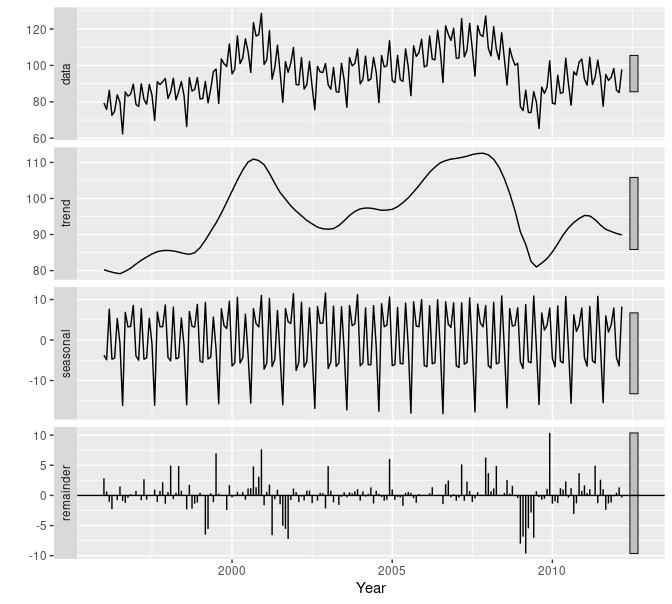
\includegraphics[width=\linewidth]{img/sota_ts_additive_decomposition.png}
		\caption{Additive decomposition of a time series using STL}
		\label{fig:stl}
	\end{figure}
	
	Given this background, let $Z=\{ z_{i, 1:T_i} \}_{i=1}^{N}$ be a  set of $N$ univariate time series where $z_{i, 1:T_i} = (z_{i,1}, z_{i,2}, ..., z_{i,T_i})$ and $z_{i,t} \in \mathbb{R}$ is the value of the $i$-th time series at time $t$. The time series in $Z$ may have different sampling frequencies, can start at different times, and may have missing values. Furthermore, let $X=\{\pmb{x}_{i, 1:T_i+\tau} \}_{i=1}^{N}$ be a set of associated, time-varying covariate vectors with $\pmb{x}_{i,t} \in \mathbb{R}^D$ being any useful information that must be known before computing the forecast up to time $T_i + \tau$ (e.g. a holiday flag).\\
	The goal of forecasting \cite{ForecastingHyndmanAthanasopoulos} is to predict the probability distribution of future values $z_{i,T_{i}+1:T_i+\tau}$ given the past values $z_{i, 1:T_i}$, the covariates $\pmb{x}_{i, 1:T_i + \tau}$, and the model parameters $\Phi$:
	\begin{equation} \label{eq:forecasting}
		p(z_{i,T_{i}+1:T_i+\tau} | z_{i, 1:T_i}, \pmb{x}_{i, 1:T_i + \tau}, \Phi)
	\end{equation}
	which, depending on the model, can be reduced to point forecast by considering the mean (e.g. $\mu$ if the model uses a Gaussian distribution), the median, or by drawing Monte Carlo samples to approximate the mean. The choice between probabilistic and point forecast depends on the application: probabilistic forecast can be used for anomaly detection or when the task has an asymmetric cost for over and under-predicting. \\
	Equation \ref{eq:forecasting} is a supervised learning problem where the model structure is usually fixed upfront and we want to learn the model parameters $\Phi$ using an optimization method such as maximum likelihood estimation.
	
	Univariate models learn the model parameters $\Phi$ for each individual time series, while multivariate models are capable of learning a single global model for multiple time series by sharing the parameters.\\
	As noted by the latest M5 competition \cite{M5Competition}, nowadays time series models are typically sufficient for identifying and capturing their historical data pattern, i.e. level, trend, and seasonality. However, relying solely on historical data fails to effectively account for the effects of holidays and special events. Moreover, such factors can affect historical data, leading to distorted time series and consequently models. In such settings, the information from exogenous/explanatory variables, i.e.  the covariates $\pmb{x}_{i, 1:T_{i+\tau}}$, becomes of critical importance to improve accuracy; in fact, recent models such as the ones discussed later \cite{FacebookProphet, DeepAR, DeepState} allow the inclusion of these kind of variables.
	
	Time series models can be categorized as generative and discriminative \cite{DiscriminativeGenerativeModels} (table \ref{table:generativediscriminative}):
	\begin{table*}\centering \label{table:generativediscriminative}
		\ra{1.3}
		\begin{tabular}{@{}rcr@{}}\toprule
			Category & Modeling\\
			 \midrule
			 Generative & $p(z_{i,1:T_i+\tau} | \pmb{x}_{i, 1:T_i + \tau}, \Phi)$\\
			 Discriminative &  $p(z_{i,T_{i}+1:T_i+\tau} | z_{i, 1:T_i}, \pmb{x}_{i, 1:T_i + \tau}, \Phi)$\\
			\bottomrule
		\end{tabular}
		\caption{Forecasting models}
	\end{table*}
	generative models assume that time series data is generated by an unknown stochastic process with some parametric structure of parameters $\Phi$ given the covariates $X$, while discriminative models model the conditional distribution for a fixed horizon $\tau$. Discriminative models are typically more flexible since they make less structural assumptions \cite{GluonTS}.
	
	
	\subsubsection{Exponential Smoothing} \label{sssec:exponential_smoothing}
	Exponential smoothing \cite{ExponentialSmoothingHoltCharles} is one of the oldest forecasting techniques that belongs to the generative models class. It is a simple and lightweight state-space model that smooths random fluctuations by using declining weights on older data, it's easy to compute and requires minimum data.
	The simplest form of exponential smoothing assumes that all past observations have equal importance:\\\\
	\centerline{$\hat{y}_{T+1} = \frac{1}{T} \sum_{t=1}^{T}y_t$}\\\\
	where $\hat{y}_{T+1}$ is the forecasted value at time $T+1$ knowing past values up to time $T$. By introducing decaying weights, the formula becomes:\\\\
		\centerline{$\hat{y}_{T+1} = A(y_T + B y_{T-1} + B^2 y_{T-2} + B^3 y_{T-3} + ...)$ }\\\\
	where $A \in [0,1]$ and $B=1-A$, $A$ can attenuate the effect of old observations. The formula can be recursively applied to obtain observation at $T+k$, $k>1$. \\
	Exponential smoothing has been extended to take into consideration linear trend and seasonality \cite{ExponentialSmoothingHoltCharles}. The trend can be approximated applying the same equation above on the time series $z_t = y_t - y_{t-1}$ while to model seasonality its period must be known beforehand.\\
	Note that due to its nature the forecasts produced by Exponential Smoothing will lag behind the actual trend.
	
	A more complex state-space approach, called Innovation State Space Model (ISSM) \cite{ExponentialSmoothingStateSpace}, has been proposed to add a statistical model that describes the data generation process, therefore providing prediction intervals. ISSM maintains a latent state vector $\pmb{l}_t$ with recent information about level, trend and seasonality which evolves over time adding a small innovation at each time step (i.e. the Gaussian noise):\\\\
	\centerline{
	$
	\pmb{l}_t = F_t \pmb{l}_{t-1} + \pmb{g}_t \epsilon_t,\; \epsilon_t \sim \mathcal{N}(0,1)
	$
	}\\\\
	where $\pmb{g}_t$ controls innovation strength and $F_t$ is the transition matrix. 
	The observations become a linear combination of the current state $\pmb{l}_t$:\\\\
	\centerline{$
	y_{t+1} = \pmb{a}_{t}^T \pmb{l}_t + b_{t} + \nu_t,\; \nu_t \sim \mathcal{N}(0,1)
	$}\\\\
	The ISSM parameters $(F_t, \pmb{g}_t, \pmb{a}_t, b_t, \nu_t)$ are typically learned using the maximum likelihood principle.
	
	\subsubsection{ARMA models} \label{sssec:arma}
	
	ARMA models are Auto-Regressive models with a Moving-Average component, they provide a complementary approach to Exponential Smoothing and they belong to the generative models class. \\
	The Auto Regressive component of order $p$, $\text{AR}(p)$, predicts the next value using a linear combination of $p$ previous known values, while the Moving Average component of order $q$, $\text{MA}(q)$, takes into consideration the average and the last $q$ differences between the predicted and the actual value.  When combined, they form an ARMA$(p, q)$ model:\\\\
	\centerline{$\hat{y}_{t} = \text{ARMA}(p, q) = \text{AR}(p) + \text{MA}(q)  = \sum_{i=1}^{p}\phi_i y_{t-i} + \mu + \epsilon_t + \sum_{i=1}^{q}\theta_i \epsilon_{t-i} $}\\\\
	Unfortunately, ARMA requires the time series to be stationary, i.e. without trends and seasonality. To make a time series stationary and apply ARMA models, Box and Jenkins \cite{BoxJenkins} proposed an approach by: (1) providing guidelines for making the time series stationary, (2)  suggesting the use of autocorrelations and partial autocorrelation for determining appropriate values for $p$ and $q$, (3) providing a set of computer programs to identify appropriate values for $p$ and $q$, and (4) estimating the parameters involved. The approach is known as the Box-Jenkins methodology to ARIMA models, where the letter \lq I \rq means ``Integrated'', reflecting the need for differencing the time series to make it stationary. Furthermore, ARIMA can deal with seasonality by applying seasonal differencing, but requires the seasonality period to be known beforehand. This extension is called SARIMA.
	
	The more general SARIMA$(p, d, q, P, D, Q, m)$ model is defined by 7 parameters:
	\begin{itemize}
		\item $p$: trend auto-regression order
		\item $d$: trend difference order
		\item $q$: trend moving average order
		\item $P$: seasonal auto-regressive order
		\item $D$: seasonal difference order
		\item $Q$: seasonal moving average order
		\item $m$: seasonal period steps
	\end{itemize}

	Besides the availability of the well defined 3-steps Box-Jenkins framework, a decent amount of human work was still required to find the right values for these parameters. To tackle this issue many approaches have been developed, some of them being made available only by commercial software.  A well known automated solution has been implemented by \cite{AutoForecasting}, where they make use of unit root tests to find the differencing orders and the Akaike's information criterion (AIC) to select the best combination of $p$, $q$, $P$, and $Q$. AIC introduces a model complexity penalty to avoid overfitting data.\\
	Nevertheless, the number of steps of the seasonal period must still be given by the analyst, although it's often a well known seasonality (e.g. daily, weekly, yearly).
		
	The vector ARIMA (VARIMA) model has been proposed as a multivariate generalization of the univariate ARIMA model, but in general Vector Auto-Regressive (VAR) models tend to suffer from overfitting, providing poor out-of-sample forecasts \cite{25YearsForecasting}.
	
	\subsubsection{ Prophet } \label{sssec:prohet}
	Prophet \cite{FacebookProphet} is a solution developed by Facebook that provides an ``analyst-in-the-loop'' approach (figure \ref{fig:analyst_in_the_loop}) and a flexible model that fit a wide range of business time series. The model simplifies the process of adding domain knowledge about the data generation process and reduces the time required to obtain high quality forecasts. Finally, Prophet is able to automatically handle time series with trend changes, multiple seasonality, and holidays effects.
	\begin{figure}
		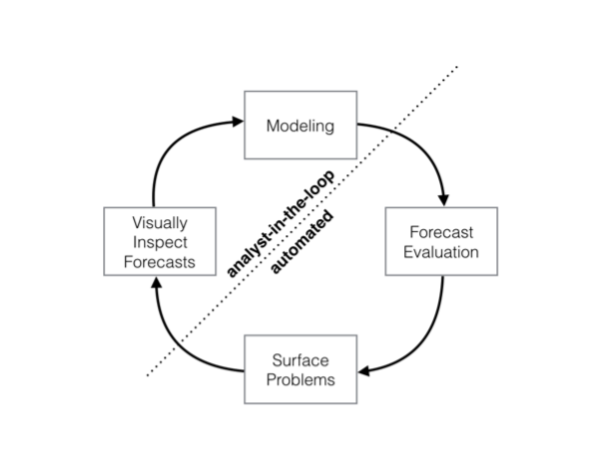
\includegraphics[width=\linewidth]{img/sota_ts_fb_prophet.png}
		\caption{Prophet analyst-in-the-loop approach}
		\label{fig:analyst_in_the_loop}
	\end{figure}
	Prophet model is a Generalized Additive Model (GAM) \cite{GAM} that decomposes trend, seasonalities, and holidays combining them in the following equation:\\\\
	\centerline{$y(t) = g(t) + s(t) + h(t) + \epsilon_t$}\\\\
	where $g(t)$ is the trend function which models non-periodic changes, $s(t)$ is the seasonality function that models periodic changes like daily and weekly seasonality, and $h(t)$ represents the effect of holidays which occur on potentially irregular schedules. Finally, the error term $\epsilon_t$ represents anything not accommodated by the model, which is assumed to be normally distributed. \\
	The GAM formulation can be easily extended to add new components as necessary and it can fit very quickly using optimization methods like L-BFGS \cite{L-BFGS}, making the forecasting problem a curve-fitting problem which allows non-regularly spaced measurements (e.g. due to missing values).\\
	The trend model $g(t)$ can be a saturating growth model capable of dealing with a limited population growth (e.g. the number of subscriptions limited by the population of a country) or a piece-wise linear model.
	The latter has the following form:\\\\
	\centerline{
		$g(t) = (k+\pmb{a}(t)^T\pmb{\delta})t + (m + \pmb{a}(t)^T\gamma)$
	}\\\\
	where $k$ is the growth rate, $\pmb{\delta}$ is the rate adjustments vector, $m$ is the offset parameter, and $\gamma_j$ is set to $-s_j\delta_j$ to make the function continuous.\\
	Therefore, $\pmb{\delta} \in \!R^S$ defines $S$ trend change points occurring at time $s_j$, with $\delta_j$ being the rate adjustment. The rate at time $t$ is $k+\sum_{j:t>s_j}\delta_j$, which is more cleanly defined by a vector $\pmb{a}(t) \in \{0,1\}^S$ such that:\\\\
	\centerline{
		$
		a_j(t) =
		\begin{cases}
			1 & \text{if $t \geq s_j$}\\
			0 & \text{otherwise}
		\end{cases}       
		$
	}\\\\
	that makes the rate at time $t$ be $k + \pmb{a}(t)^T\pmb{\delta}$\\
	The change points $s_j$  can be specified by the analyst or they can be automatically selected by putting a sparse prior on $\pmb{\delta}$, e.g. a Laplace prior.\\
	The seasonality function $s(t)$ is modeled using Fourier series, meaning that a seasonality with period $P$ can be approximated by:\\\\
	\centerline{$s(t) = \sum_{n=1}^{N} (a_n \cos{(\frac{2\pi nt}{P})} + b_n \sin{(\frac{2\pi nt}{P})}) $}\\\\
	which can be automatically estimated finding $2N$ parameters, i.e.\\ $ \pmb{\beta} =  (a_1, b_1, ..., a_N, b_N)$. By choosing $N$, the series can be truncated at different depths allowing to fit seasonal patterns that change more or less quickly, possibly leading to overfitting. Finally, the initialization $\pmb{\beta} \sim \mathcal{N}(0, \sigma^2)$ allows to impose a prior on the seasonality by choosing $\sigma$. \\
	The holiday model $h(t)$ can deal with predictable shocks that cannot be modeled by a smoothed Fourier series.  An example could be the increase of units sold during Easter, which doesn't falls a specific day. An analyst can provide a list of dates of interest $D_j$ for each holiday $j$, so the holiday model becomes:\\\\
	\centerline{$h(t) = Z(t) \pmb{\kappa}$}\\\\
	with $Z(t) = [ \mathbf{1} (t \in D_1), ..., \mathbf{1} (t \in D_L)] $ and $\pmb{\kappa}$ initialized as $\pmb{\kappa} \sim \mathcal{N}(0, v^2)$, like it was done with seasonality.\\
	The Prophet solution is capable of achieving lower prediction errors when compared to traditional methods like Exponential Smoothing and ARIMA, with very quick fitting time.
	
	\subsubsection{ML models}
	The forecasting field has seen past practitioners proposing novel Neural Networks (NN) architectures that could not be considered competitive against simpler univariate statistical models. However, we are now living in the Big Data era: companies have gathered huge amounts of data over the years containing important information about their business patterns, unlocking the possibility of learning effective multivariate models. Big data in the context of time series doesn't necessarily mean having single time series with with a lot of historical data, but it rather means that there are many related time series from the same domain \cite{RNNForecasting}. In such context, models capable of learning from multiple time series have emerged \cite{M5Competition} outperforming traditional ones while alleviating the time and labor intensive manual feature engineering by making no explicit assumptions on data and therefore being more flexible when compared to traditional techniques such as ARIMA and Exponential Smoothing.
	
	All recent successful models are based on Recurrent Neural Networks (RNN) \cite{RNN, RNNForecasting}, which demonstrated state-of-the-art performance in various applications handling sequential data like text, audio, and video where some kind of state must be kept while processing. RNNs can be combination of recurrent units like Long Short-Term Memory (LSTM) and Gated Recurrent Unit (GRU) (see figure \ref{fig:lstmgru}). 
	\begin{figure}
		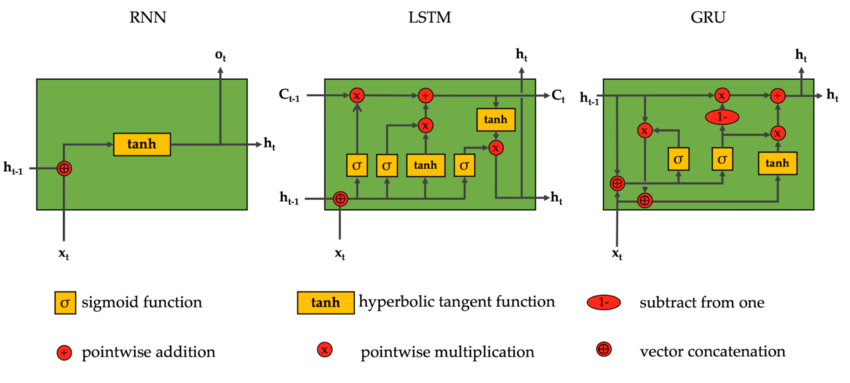
\includegraphics[width=\linewidth]{img/rnns.png}
		\caption{Architecture of an Elman recurrent unit, LSTM, and GRU. The output at step $t-1$ influences the output at step $t$.}
		\label{fig:lstmgru}
	\end{figure}
	By using recurrent edges connecting adjacent time steps (i.e. feedback loops), RNNs introduce the notion of time to the model: at time step $t$ the network receives the current input $\pmb{x}^{(t)}$ plus the previous network state $\pmb{h}^{(t-1)}$ producing a new context $\pmb{h}^{(t)}$ (often called hidden state) and eventually an output $\pmb{o}^{(t)}$.
	The context acts as a memory of what the network has seen so far and influences the output, unlocking a stateful decision making.\\
	However, the first recurrent unit (i.e. the Elman recurrent unit) suffered from the vanishing/exploding gradient problem \cite{VanishingGradient} which causes the inability of carrying long-term dependencies. To address this shortcoming, the Elman recurrent unit has been extended leading to improved variants such as LSTM and GRU.
	
	LSTM uses two components for its state: the hidden state and the internal state, containing short-term and long-term memory respectively. Furthermore, LSTM introduces a gating mechanism made of an input, forget, and output gate used to filter what should or should not be kept of the state in the next step (for example, to disable the output contribution to the LSTM state just set the output gate to zero). GRU is a simpler version of LSTM with fewer gates (update and reset) which allows faster computations and is less prone to overfitting due to the lower number of parameters.
	
	Recurrent units (e.g. LSTM, GRU) can constitute RNNs in various types of architectures, depending on the application: a many-to-one (or sequence-to-vector) architecture can be used for sentiment classification, one-to-many (or vector-to-sequence) for for music generation, and many-to-many (or sequence-to-sequence) for machine translation (see figure \ref{fig:rnn_architectures}).
	\begin{figure}
		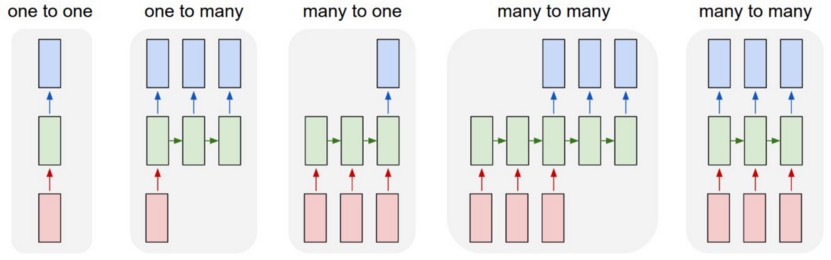
\includegraphics[width=\linewidth]{img/rnn_architectures.png}
		\caption{RNN architectures. Red rectangles are input vectors, blue rectangles are output vectors, and green rectangles are recurrent units such as LSTM or GRU which share the same weights while their state evolves from left to right.}
		\label{fig:rnn_architectures}
	\end{figure}

	To obtain such architectures a single LSTM can be used, in that case the green LSTM in figure \ref{fig:rnn_architectures} is unfolded such that in the whole processing of the input the same weights are used, while the internal state of the LSTM evolves.	Nevertheless, multiple LSTMs can be stacked together such as in figure \ref{fig:stacked_lstm} composing multiple layers and increasing the expressiveness of the network.
	\begin{figure}
		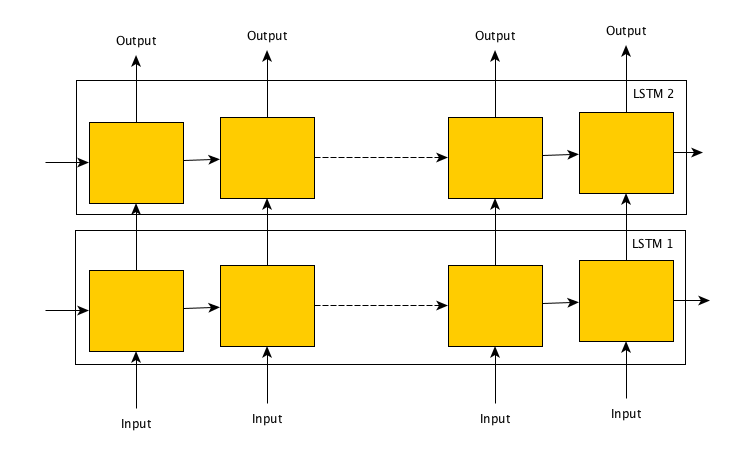
\includegraphics[width=\linewidth]{img/stacked_lstm.png}
		\caption{2-layers stacked LSTMs. }
		\label{fig:stacked_lstm}
	\end{figure}
	Usually when forecasting the size $d$ of the output (or the internal state of an LSTM) doesn't match the dimension of the forecasting horizon $H$. In such cases, another neural layer is added to map $\pmb{o}^{(t)} \in \mathbb{R}^d$ to the forecast $\hat{\pmb{y}}^{(t)} \in \mathbb{R}^H$. This neural layer is trained together with the LSTM, with the loss (e.g. the forecasting error $|\hat{y} - y|$) being calculated per each time step and accumulated until the end of the time series after which backpropagation through time is executed.
	
	Forecasting requires a many-to-many architecture: the input is a sequence, i.e. a time series, and the output is another sequence that is a continuation of the input sequence, i.e. a forecast of horizon $H$. In such context, the Sequence to Sequence (S2S) \cite{seq2seq} models have proven to be successful. S2S models are made of two RNNs: an encoder followed by a decoder, as shown in figure \ref{fig:seq2seq}.
	\begin{figure}
		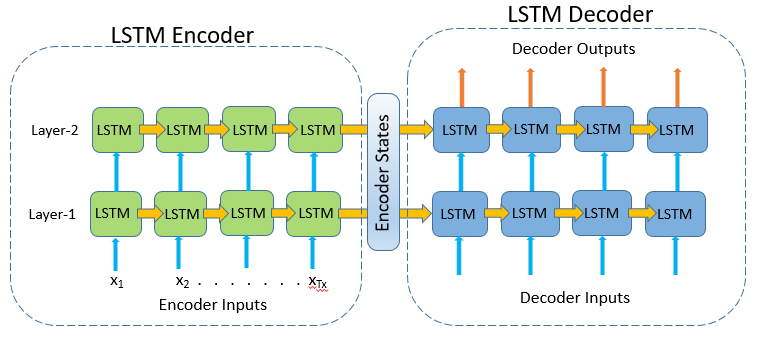
\includegraphics[width=\linewidth]{img/seq2seq.png}
		\caption{Sequence to sequence model}
		\label{fig:seq2seq}
	\end{figure}
	 The encoder is used to extract features from known time series data in order to produce a context vector (e.g. the LSTM hidden state) that is given as input to the decoder to produce forecasts. Examples of models based on S2S are DeepAR \cite{DeepAR} and Multi-Horizon Quantile Recurrent Forecaster \cite{MQCNN}, explained later. By defining an encoder and a decoder, a model is allowed to see a limited amount of past values and can predict a fixed horizon, which means that any context and prediction length change requires re-training. 
	 
	 The decoder at time step $t+1$ can receive as input the prediction made at step $t$, but many forecasting problems have long periodicity (e.g. 365 days) and may suffer memory loss during forward propagation. To overcome the long-term dependency issue \cite{NARX} proposed a recurrent unit which computes a hidden state $\pmb{h}^{(t)}$ not only based on previous state $\pmb{h}^{(t-1)}$ but also a specific set of other past states (e.g. $(\pmb{h}^{(t-2)}), ..., \pmb{h}^{(t-D)})$) facilitating the ability of keeping long dependencies. This technique is called skip-connection. However, the naive alternative adopted by \cite{DeepAR, MQCNN} obtains the same effect by directly feeding past time series values $(y_{t-1}, ..., y_{t-D})$ as feature inputs to the decoder.
	
	More generally, the idea of feeding both time-dependent and time-independent features as input (often called exogenous variables), along with the time series data points, has proven to be successful: when dealing with huge datasets, assigning time-independent (or static) features such as the category of the time series (e.g. ``clothing'' in the context of shopping) allow the model to learn both global and category-specific patterns, while time-dependent (or dynamic) features like day of week, holidays, and relevant events allow the model to learn and distinguish seasonality patterns from one-shot events like anomalies, reducing the risk of overfitting. However, such dynamic features must be known beforehand when computing forecasts, and in some contexts they can be used to make conditional forecasts, e.g. "\textit{How many units of product X will I sell if I set the price to Z?}".
	
	The usage of such combination of features facilitates the learning of a global model exploiting information from many time series simultaneously. For NNs this means that weights are learned globally, but the state is maintained for each time series. Furthermore, the global model can be used to forecast time series that have never been seen during training and lack of data, as the model can still use patterns learned from the training set.
	
	
	
	
	% TODO introduction about RNNs - characteristics e.g. of LSTM - see https://arxiv.org/pdf/1705.04378.pdf , background of https://arxiv.org/pdf/1703.04691.pdf
	\subsubsection{ DeepAR } \label{sssec:deepar}
	DeepAR \cite{DeepAR} is a discriminative model capable of probabilistic forecasts in the form of Monte Carlo samples, it is based on Sequence to Sequence (S2S) \cite{seq2seq} and can learn a global model from multiple time series.\\
	Alongside with a model, DeepAR proposes a solution to the issue of dealing with time series having very different magnitudes, which are known to ruin the learning of an effective global model reducing the effectiveness of normalization techniques on some datasets \cite{DeepAR}.
	
	DeepAR goal is to model the conditional distribution\\\\
	\centerline{
	$
	P(\pmb{z}_{i, t_0:T} | \pmb{z}_{i, 1:t_0-1}, \pmb{x}_{i, 1:T})
	$
	}\\\\
	where $\pmb{z}_{i, t_0:T} = [z_{i,t_0}, z_{i, t_0+1}, ..., z_{i, T}]$ is the future (or prediction range), $\pmb{z}_{i, 1:t_0-1}$ is the past (or conditioning range), and $\pmb{x}_{i, 1:T}$ are covariates that must be known for all time points.
	
	DeepAR assumes that its distribution $Q_{\Theta}(\pmb{z}_{i, t_0:T} | \pmb{z}_{i, 1:t_0-1}, \pmb{x}_{i, 1:T})$ consists of a product of likelihood factors:\\\\
	\centerline{
	$
	Q_{\Theta}(\pmb{z}_{i, t_0:T} | \pmb{z}_{i, 1:t_0-1}, \pmb{x}_{i, 1:T}) 
	= \prod_{t=t_0}^{T} Q_{\Theta}(z_{i, t} | \pmb{z}_{i, 1:t-1}, \pmb{x}_{i, 1:T})
	= \prod_{t=t_0}^{T} \textit{l}(z_{i,t} | \theta(\pmb{h}_{i,t}, \Theta))
	$
	}\\\\
	which is parametrized by the output $\pmb{h}_{i,t}$ of an autoregressive RNN
	\begin{equation} \label{eq:autoregressive_rnn}
		\pmb{h}_{i,t} = \textit{h}(\pmb{h}_{i,t}, \pmb{z}_{i, t-1}, \pmb{x}_{i, t}, \Theta )
	\end{equation}
	where \textit{h} is implemented by multi-layer RNN with LSTM cells, meaning that $\pmb{h}_{i,t}$ is given by the internal state of the LSTMs as shown in figure \ref{fig:deepar}. \\
	$\textit{l}(z_{i,t} | \theta(\pmb{h}_{i,t})$ is the likelihood of a fixed distribution (e.g. Student's t-distribution) whose parameters are given by a function $\theta(\pmb{h}_{i,t}, \Theta)$ of the network output $\pmb{h}_{i,t}$.
	\begin{figure}
		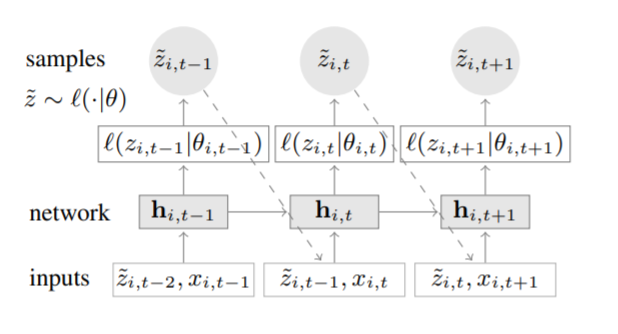
\includegraphics[width=\linewidth]{img/deepar.png}
		\caption{DeepAR decoder network}
		\label{fig:deepar}
	\end{figure}
	The model is autoregressive and recurrent as it uses the previous output $\tilde{z}_{i,t}$ and state $\pmb{h}_{i,t}$ as input, which potentially means that prediction errors at time $t$ will negatively affect predictions at time $t>1$. \\
	The initial state $\pmb{h}_{i,t_0-1}$ of the decoder shown in figure \ref{fig:deepar} is obtained using an encoder with the same architecture and weights that computes equation \ref{eq:autoregressive_rnn} for $t = 1, ..., t_0-1$. The forecasts $\tilde{\pmb{z}}_{i, t_0:T}$ are obtained by sampling $\tilde{z}_{i,t} \sim l(\cdot | \theta(\pmb{h}_{i,t}, \Theta))$, where $\theta(\pmb{h}_{i,t}, \Theta))$ are the parameters (e.g. mean and variance) of the distribution fixed during training and are directly predicted by the decoder network.
	
	The likelihood $l(z | \theta)$ determines the noise model and should match the statistical properties of the data: a Gaussian likelihood can be used for real-valued data, a beta likelihood for data in the unit interval, and a negative-binomial likelihood for positive count data. For example, the Gaussian likelihood is parametrized using its mean and standard deviation, i.e. $\theta = (\mu, \sigma)$ where $\mu$ is obtained with an affine function of the network output $\pmb{h}_{i,t}$ and the standard deviation is obtained by applying an affine transformation followed by a softplus activation to ensure $\sigma > 0$,
	Therefore, each likelihood with parameters $\theta$ requires a mapping from the decoder state $\pmb{h}_{i,t}$ to $\theta$ whose parameters are learned by the network.
	
		Without any modification, in order to handle different scales the network should learn to scale the input to an appropriate range and then invert the scaling. As the network has a limited operating range and some datasets exhibit a power-law of scales (such as the Amazon dataset of \cite{DeepAR}), this issue was addressed by scaling the input values (e.g. $\tilde{z}_{i, t}$ and $z_{i,t}$) using an item-dependent factor $\nu_i$. Then, before drawing samples from the distribution, the output of the network (e.g. the mean $\mu$ of the Gaussian) is multiplied by the scale. The scaling factor $\nu$ is set to be the average value of the time series: $\nu_i = 1 + \frac{1}{t_0} \sum_{t=1}^{t_0} z_{i,t}$. Finally, rather than training the network choosing random time series from the dataset, the probability of choosing a time series is proportional to its scale factor $\nu_i$: by non-uniformly sampling during training, imbalanced datasets with fewer large scale time series are used more effectively.
		
	
	\subsubsection{ DeepState } \label{sssec:deepstate}
	DeepState \cite{DeepState} is a generative model that combines state space models \cite{ExponentialSmoothingStateSpace} with deep learning. The idea is to use a latent state $\pmb{l}_t \in \mathbb{R}^D$ to encode time series components such as level, trend, and seasonality patterns, and parametrize the linear state space model (SSM) by using a recurrent neural network (RNN) whose weights are learned jointly from multiple time series and covariates. \\
	The main advantage of SSM is that the model is easily interpretable, but when used with traditional models such as ARIMA and Exponential Smoothing it results in an univariate model that still requires a lot of human work that cannot be easily recycled for other time series.
	DeepState solves this issue by using neural networks to learn a global model from multiple time series without making strong assumptions and reducing the human effort, and solving the common interpretability issue of neural networks by fusing them with SSMs.
	
	The goal of DeepState is to produce probabilistic forecasts for each time series $i=1,...,N$ given the past:\\\\
	\centerline{
	$
	p(\pmb{z}_{i, T_i+1:T_i+\tau}| \pmb{z}_{i, 1:T_i}, \pmb{x}_{i, 1:T_i+\tau}; \Phi)
	$
	}\\\\
	where $\pmb{z}_{i, T_i+1:T_i+\tau}$ are the $\tau$ future values, $ \pmb{z}_{i, 1:T_i}$ are the known past values, $\pmb{x}_{i, 1:T_i+\tau}$ are the covariates that must be known beforehand for $t=1,...,T$, and $\Phi$ is the set of learnable parameters of the model (i.e. the RNN).\\
	DeepState makes the assumption that time series are independent of each other when conditioned on the associated covariates $\pmb{x}_{i, 1:T}$. Nevertheless, the model is still able to learn and share patterns across time series as $\Phi$ is shared (and learned) between all of them.
	
	SSMs use a latent state $\pmb{l}_t \in \mathbb{R}^L$ encoding time series components (level, trend, seasonality) that evolves over time with linear transitions at each time step $t$:\\\\
	\centerline{
	$
	\pmb{l}_t = F_t \pmb{l}_{t-1} + \pmb{g }_t \epsilon_t, \;\; \epsilon_t \sim \mathcal{N}(0,1)
	$
	}\\\\
	where $F_t$ is the transition matrix and $\pmb{g }_t \epsilon_t$ is a random innovation component. The latent state can be inspected to check and potentially change the encoded trend and seasonality, and is also used to obtain predictions. For example, considering a linear Gaussian observation model:
	\begin{equation} \label{eq:deepstate}
			z_t = y_t + \sigma_t \epsilon_t, \;\; y_t = \pmb{a}_t^T \pmb{l}_{t-1} + b_t, \;\; \epsilon_t \sim \mathcal{N}(0,1)
	\end{equation}
	with the initial state $\pmb{l}_0 \sim \mathcal{N}(\pmb{\mu}_0, \text{diag}(\pmb{\sigma}_0^2))$, $\pmb{a}_t \in \mathbb{R}^L$, $\sigma_t \in \mathbb{R}_{>0}$, and $b_t \in \mathbb{R}$ varying over time. \\
	Therefore, the state space model of \textit{one} time series is fully described by $\Theta_t = (\pmb{\mu}_0, \pmb{\sigma}_0, \pmb{F}_t, \pmb{g}_ t, \pmb{a}_t, b_t, \sigma_t), \; \forall t > 0$, differing from the classical settings where $\Theta$ doesn't change with time.\\
	To obtain $\Theta_{i,t}$ for the time series $i$, the DeepState model learns a mapping $\Psi$ from the covariates $\pmb{x}_{i, 1:T_i}$ to the parameters $\Theta_{i, t}$:\\\\
	\centerline{
	$
	\Theta_{i,t} = \Psi(\pmb{x}_{i, 1:T}, \theta)
	$
	}\\\\
	that is parametrized from a set of parameters $\theta$ learned jointly from the entire dataset of time series. \\
	More precisely, the mapping $\Psi$ is implemented by the RNN shown in figure \ref{fig:deepstate} having a stacked architecture of LSTM cells. Its parameters $\theta$ are learned by maximizing the likelihood during training.
	\begin{figure}
		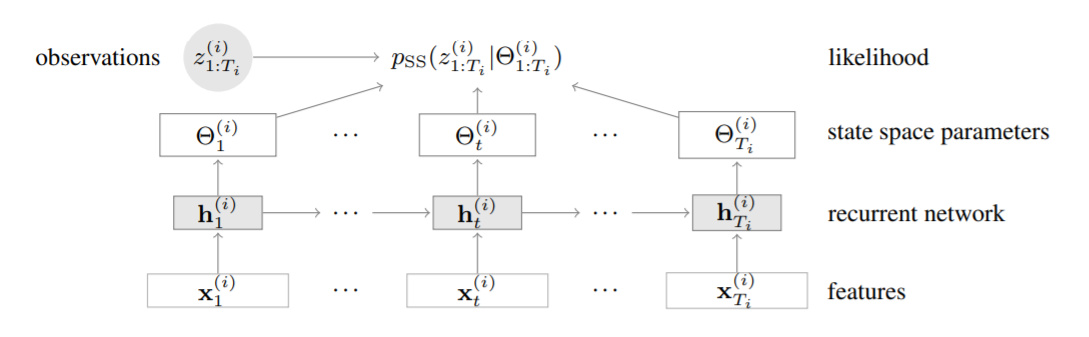
\includegraphics[width=\linewidth]{img/deepstate.png}
		\caption{DeepState network}
		\label{fig:deepstate}
	\end{figure}

	Finally, once the mapping is learned and given $\pmb{x}_{i, 1:T_i}$, the data $\pmb{z}_{i,1:T_i}$ is distributed according to the marginal likelihood:\\\\
	\centerline{
	$
	p(\pmb{z}_{i, 1:T_i} | \pmb{x}_{i, 1:T_i}, \theta)
	= p_{SS}(\pmb{z}_{i, 1:T_i} | \Theta_{i,1:T_i})
	$
	}\\\\
	\centerline{
		$
		= p(z_{i,1} | \Theta_{i,1}) \prod_{t=2}^{T}p(z_{i,t} | z_{i, 1:t-1}, \Theta_{i, 1:t})
		$
	}\\\\
	\centerline{
		$
		= \int p(\pmb{l}_0) [\prod_{t=1}^{T_i} p(z_{i,t} | \pmb{l}_t)p(\pmb{l}_t | \pmb{l}_{t-1})] d\pmb{l}_{0:T_i}
		$
	}\\\\
	that is analytically tractable in the linear-Gaussian case.\\
	To produce a forecast, the posterior of the last latent state $p(\pmb{l}_T | z_{i, 1:T_i})$ is computed using the observations $z_{i, 1:T_i}$, then the RNN is fed with the covariates $x_{i, 1:T_i+\tau}$ (see figure \ref{fig:deepstate2}) while the transition equation is recursively applied, drawing Monte Carlo samples using equation \ref{eq:deepstate}.
	\begin{figure}
		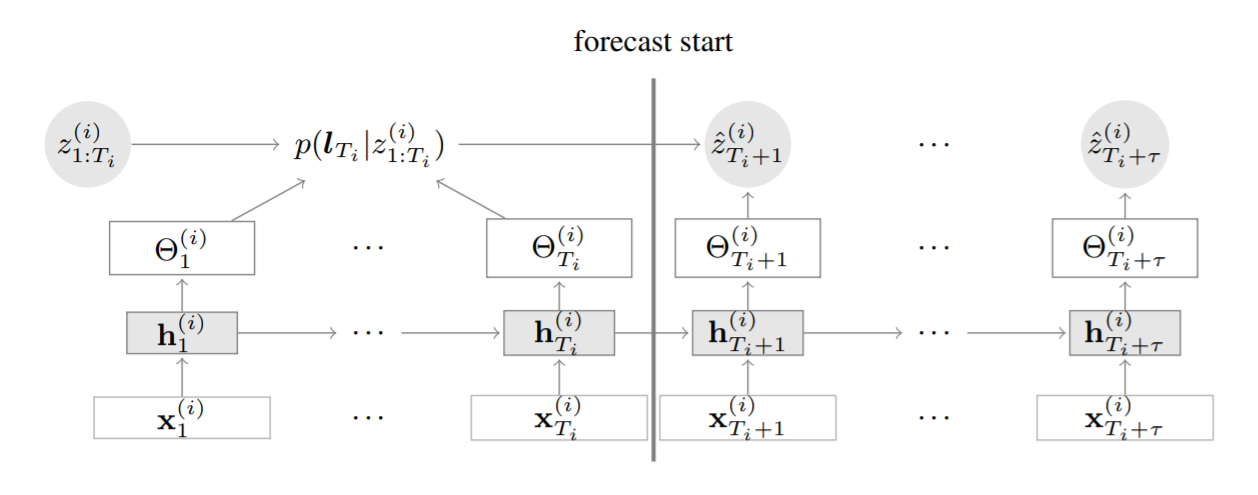
\includegraphics[width=\linewidth]{img/deepstate2.png}
		\caption{DeepState forecast illustration}
		\label{fig:deepstate2}
	\end{figure}

	\subsubsection{ Multi Quantile Recurrent Forecaster } \label{sssec:mqcnn}
	Multi Quantile Recurrent Forecaster (MQCNN) \cite{MQCNN} is a Sequence-to-Sequence RNN-based model capable of producing multi-horizon quantile forecasts.\\
	\cite{MQCNN} proposes a forking-sequences approach that improves the training stability and performance of encoder-decoder architectures by efficiently training on all time points where a forecast could be created. Furthermore, the model can be used with different encoders, but the best results were achieved using a CNN-based encoder.
	
	To train a quantile regression model for a quantile $q \in [0, 1]$ the loss of a single forecasted value is given by:\\\\
	\centerline{
	$
	L_q(y, \hat{y}) = q \max(0, y-\hat{y}) + (1-q) \max(0, \hat{y} - y)
	$
	}\\\\
	where by setting $q=0.5$ the model will be trained to simply predict the median. Note that by predicting quantiles the model is robust since it doesn't make distributional assumptions (e.g. like DeepAr \cite{DeepAR}). \\
	Eventually, more quantiles can be considered such that the total loss is given by:\\\\
	\centerline{
	$
	\sum_{t\in T} \sum_{q\in Q} \sum_{k=1}^K L_q(y_{t+k}, \hat{y}_{t+k}^{(q)})
	$
	}\\\\
	where $T$ contains the forecast creation times, $Q$ the quantiles, and $K$ is the size of the horizon to forecast. Furthermore, different quantiles can be associated with different weights, which could be useful for tasks with an asymmetric cost for over and under-predicting.
	
	The general architecture of a multi-quantile recurrent forecaster is shown in figure \ref{fig:mqforecaster}. 
	\begin{figure}
		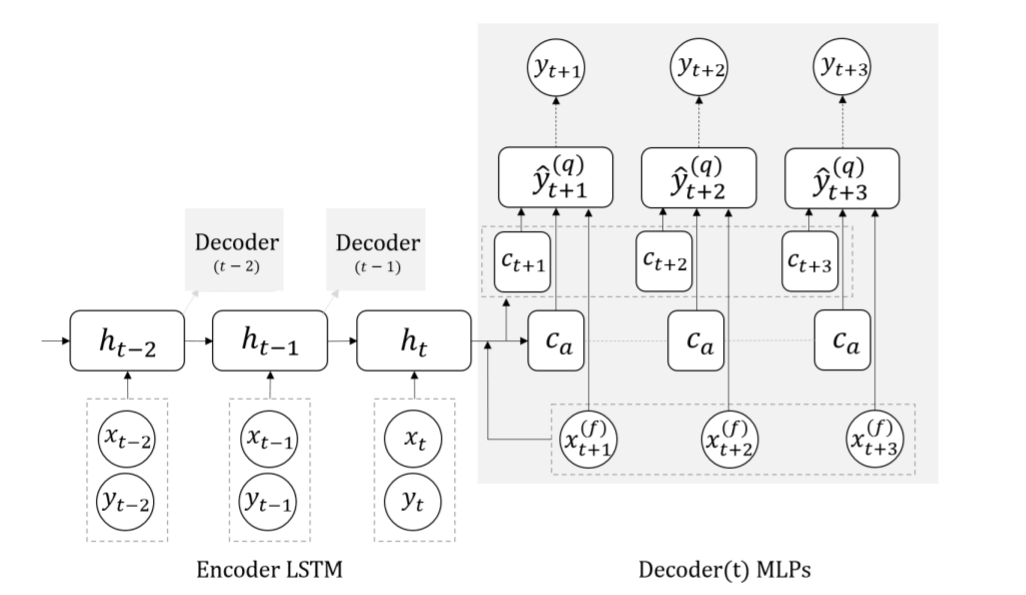
\includegraphics[width=\linewidth]{img/mqcnn.png}
		\caption{Multi-quantile recurrent forecaster architecture}
		\label{fig:mqforecaster}
	\end{figure}
	The encoder is fed with the time series history producing hidden states $h_t$,  then a global neural network summarizes the encoder output into an horizon-agnostic context $c_a$ plus a horizon-specific context $c_{t+k}$ for $k=1,...,K$ using the hidden state $h_t$ and the future covariates $x_{t+1:t+K}$:\\\\
	\centerline{
	$
	(c_{t+1, ..., c_{t+K}, c_a}) = m_G(h_t, x_{t+1:t+K})
	$
	}\\\\
	where each context $c_i$ can have arbitrary dimension. The idea behind this choice is that $c_a$ should capture relevant information that is not time-sensitive, while $c_{t+k}$ carries awareness of the temporal distance between the forecast creation time $t$ and the specific horizon.\\ 
	Then, these contexts are used by a local neural network to compute the quantiles of a specific horizon $t+k$ for each $k=1,...,K$ using the horizon-agnostic context and the horizon-specific context, plus the associated covariates:\\\\
	\centerline{
	$
	(\hat{y}_{t+k}^{(q_1)}), ..., \hat{y}_{t+k}^{(q_Q)}) = m_L(c_{t+k}, c_a, x_{t+k})
	$
	}\\\\
	The local neural network implementing $m_L$ has its parameters shared across all the horizons.
	
	The motivation for replacing the standard RNN-based decoder is that the horizon-specific context should have already captured the flow of temporal information. Furthermore, by not feeding predictions recursively there is no error accumulation and following the forking-sequences training scheme proposed by \cite{MQCNN} the training time is dramatically reduced while the process of updating the gradients is stabilized, leading to better forecasts with a reduced effort.
	
	The encoder is not limited to be a simple LSTM-based RNN: \cite{MQCNN} achieved the best results using a CNN-based encoder made of a stack of dilated causal convolutional layers, similarly to the work done by WaveNet \cite{Wavenet}.\\
	Dilated causal convolutional layers, shown in figure \ref{fig:dilated_cnn}, form long-term connections creating large receptive fields with just a few layers, thus preserving computational efficiency. The result is the so-called MQ-CNN model.
	\begin{figure}
		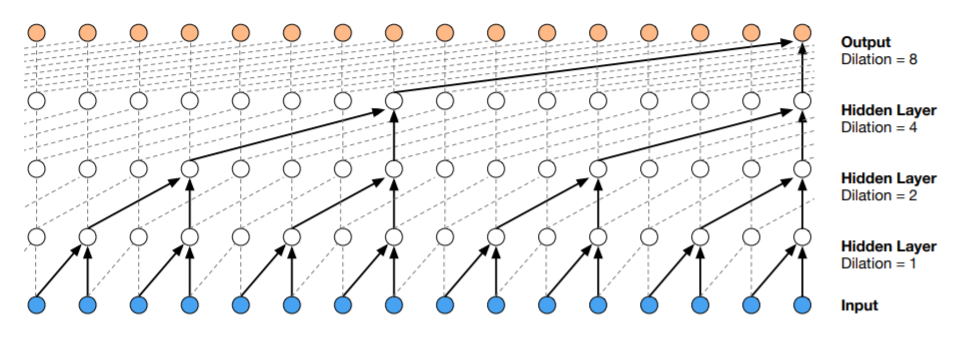
\includegraphics[width=\linewidth]{img/wavenet.png}
		\caption{A stack of dilated causal convolutional layers}
		\label{fig:dilated_cnn}
	\end{figure}
	
	
	\subsection{ Workload forecasting } \label{ssec:workload_forecasting}
	% ADD stuff about short term load forecasting (STLF) see https://arxiv.org/pdf/1705.04378.pdf
	The ability of forecasting the workload of an IT system opens the possibility of adapting the system according to the future demand and making smarter decisions, keeping the Quality of Service (QoS) high while reducing the infrastructure costs. This section lists some applications of workload forecasting and how it is often approached.\\
	Recent years have seen companies moving from self-hosted to cloud-hosted  IT services, where a public provider is paid to lend on-demand computing power likewise utilities such as electricity, gas, and water. This paradigm, called cloud computing \cite{CloudComputing}, enabled the possibility of flexibly adapting the capacity of a system according to the demand, potentially heavily reducing the infrastructure costs. \\
	A scalable system can acquire new resources in a matter of minutes, thus quickly reacting to changes in the demand. However, the demand a system is subject to can as quickly increase, making a reactive approach often inappropriate due to spikes in the demand that can cause disservices or even system crashes \cite{ArimaWorkloadPrediction}, leading to a loss of customers. In this context, a workload forecasting module that can make reliable forecasts about the upcoming workload allows to proactively adapt the system, reducing costs while providing high QoS. Such module must predict the workload by modeling time series with sub-hourly frequencies, representing metrics such as CPU usage and number of incoming requests.\\
	To do so, \cite{ArimaWorkloadPrediction} used ARIMA to predict the number of end-users' future requests to meet the QoS targets while reducing the resources utilization, focusing on specific request patterns that exhibit seasonal behavior. \cite{ArmaAutoscaling} used ARMA models to predict the upcoming workload and proactively autoscale the IT system under study, focusing on a small number of machines and leaving the exploration of the feasibility of their solution with modern workloads and large number of resources for future work.
	In order to deal with huge numbers of machines, with the goal of efficiently provision computing resources in the cloud, \cite{WorkloadCharacterizationAndPrediction} adopted the approach of first grouping machines with high correlation and then making predictions about individual machine's workload based on the groups found on the previous step using Hidden Markov Model. 
	\cite{LSTMLargeScaleWorkloadForecasting} proposes the usage of LSTM-based neural networks to forecast the workload in large-scale computing centers, highlighting that training models on one-dimensional time series doesn't capture useful similarities across multiple time series. 
	
	Another task that makes use of workload forecasting is job scheduling. In the context of cloud service providers, running database backups while there are peaks of customer activity results in inevitable competition for resources and poor QoS. \cite{Seagull} proposed an automated solution to schedule backups during intervals of minimum activity comparing the forecasting models proposed by \cite{MicrosoftSSA, GluonTS, FacebookProphet} in terms of accuracy and scalability. Interestingly, they discarded the ARIMA model due to its long execution time. Furthermore, by analyzing the typical customer activity patterns on PostgreSQL and MySQL servers, \cite{Seagull} discovered that the majority of the activity can be classified either as stable or as a daily or weekly pattern: less than 1\% of the servers didn't follow either a daily or weekly pattern.
	
	The application of novel forecasting techniques such as the ones based on neural network has still to be explored. Nevertheless, the flexibility of such models, especially when compared to ARIMA and Exponential Smoothing, is promising: potentially dealing with huge numbers of time series with minimum effort, while keeping the forecasting accuracy high, would make workload forecasting much more accessible to many companies, leading to better services and lower costs.
	
	\section{ Proposed solution and approach }
	At the time of writing, Akamas \cite{AkamasCGP} optimizes IT systems on a staging environment (a replica of the real system) using artificial workloads that have no impact on the user experience. The goal of this work is to extend the underlying tuner so it can be applied to the actual IT system running under the real workload, with the advantages of reducing the effort explained in section \ref{ssec:workload_characterization} and obtaining performance measurements directly from the ``real'' system. To do so, as explained in section \ref{ssec:contextual_bayesian_optimization}, we need a workload characterization and a workload forecasting module.
	
	The main challenge when tuning a system while it is serving its clients is to keep QoS levels high, and at the same time quickly finding good configurations for the system. Furthermore, we want Akamas to be easy to configure and apply in order to require the minimum amount of human work. Therefore, the requirements for the solution are to be autonomous and reliable.
	
	The autonomous requirement translates to the need of a workload forecasting module that can train good models without having to inspect the time series composing the workload, and possibly without having inject domain knowledge about the system being optimized. The reliability requirement requires the models to be as accurate as possible. Furthermore, as the solution is running in real-time, it must be possible to train the forecasting models in a decent amount of time in order to incorporate new data, and the prediction queries must be satisfied in a matter of seconds.
	
	As stated in section \ref{ssec:contextual_bayesian_optimization}, we are interested in finding short time windows during which the workload will be stable, along with the average values the workload time series will assume. \\
	Formally, given the forecast $\tilde{Y}_{t_1:t_2} = (\tilde{\pmb{y}}_{t_1:t_2}^1, ..., \tilde{\pmb{y}}_{t_1:t_2}^n)$ at time $t$, where $\tilde{\pmb{y}}_{t_1:t_2}^i, \; i\in [1, n]$ is the forecast of the $i$-th time series composing the workload, we want to know if the window $\omega_{t_1:t_2}$ assuming values $\tilde{Y}_{t_1:t_2}$, starting at time $t_1 \geq t$ and ending at time $t_2 > t_1$ is stable: 
	\begin{equation}
		s_\Theta(\tilde{Y}_{t_1:t_2}, Y_{t_0:t_1}) = \begin{cases}
			1 & \text{if $\tilde{Y}_{t_1:t_2}$ is stable}\\
			0 & \text{otherwise}
		\end{cases}    
	\end{equation}
	where $s_\Theta$ is a function with hyper-parameters $\Theta$ that marks whether a forecasted window is stable or not, given the historical values $Y_{t_0:t_1}$. The forecast $\tilde{Y}_{t_1:t_2}$ is also used by the tuner to suggest a workload-tailored configuration.
	To obtain such forecast, the forecasting module explained in section \ref{ssec:forecasting_module} was developed, while the component developed to implement the function $s_\Theta$ is detailed in section \ref{ssec:stable_window_finder}. Finally, the workload characterization module is presented in section \ref{ssec:workload_characterization_module}. 
	
	\subsection{Online Contextual Gaussian Process Tuner}
	Before starting the tuning process, made of iterations (or experiments) where a new configuration is repeatedly applied and evaluated, we must collect enough workload data in order to train the forecasting models and gather knowledge about the workload (see section \ref{ssec:workload_characterization_module} for details).
	As stated by \cite{Seagull}, a significant number of workloads follow a daily or a weekly seasonality. Therefore, the data collection time lasts at least one week.
	 
	 After the collection period has ended, the online tuning process of the IT system can start. The tuning process is made of experiments of duration up to $t_2 - t_1$, that is the length of the window $\omega_{t_1:t_2}$ on which a configuration is applied and its outcome is measured.  However, it can happen that an experiment gets invalidated due to an early stop condition such as the violation of constraint (TODO add ref to cgp explaining violations).  
	 
	 After a forecast is made, the experiment develops and the true workload reveals itself. When comparing the predicted with the actual workload, two (bad) cases can occur: the predicted average workload is different from the true average workload, and the stability prediction is not correct (e.g. predicted stable but it is unstable). The latter case is further detailed by the four sub-cases shown in table \ref{table:stability_cases}. 	 
	 \begin{table*}\centering \label{table:stability_cases}
	 	\ra{1.3}
	 	\begin{tabular*}{\textwidth}{@{}rcr@{}}
	 		\toprule
	 		Case & Outcome\\
	 		\midrule
	 		Predicted stable, revealed stable (TP) & Experiment opportunity taken\\
	 		Predicted stable, revealed unstable (FP)& Experiment failed\\
	 		Predicted unstable, revealed unstable (TN)& Experiment not available\\
	 		Predicted unstable, revealed stable (FN)& Experiment opportunity lost\\
	 		\bottomrule
	 	\end{tabular*}
	 	\caption{Window stability outcomes. TP, FP, TN, FN stands for True Positive, False Positive, True Negative, and False negative respectively.}
	 \end{table*}
	 The most dangerous case occurs when we predict that the workload is going to be unstable but actually it won't (i.e. false positive case): in such case, the tuner may suggest a configuration that leads to low QoS, ruining user experience. However, if we miss a stable window (i.e. false negative case), we just lengthened the tuning process.
	 In case of false positives we chose to discard the experiment: its evaluation requires us to measure the average performance of the configuration, and an unstable workload may lead to unrealistic measurements.\\
	 Similarly, we could face issues if the predicted and true windows are stable, but the actual average workload differs from the real average. In such cases, we still consider the experiment valid as it can provide useful information to the tuner.
	 
	 In summary, each experiment is made of the following steps: 
	\begin{enumerate}
		\item Forecast the upcoming workload $\tilde{Y}_{t_1:t_2}$.
		\item Apply $s_\Theta(\tilde{Y}_{t_1:t_2}, Y_{t_0:t_1})$ to find whether the upcoming workload $\tilde{Y}_{t_1:t_2}$ is stable.
		\item If the upcoming workload is predicted to be unstable stop the experiment and go back to step 1, otherwise continue.
		\item Ask the tuner a new configuration $x$ given the average of the predicted workload $\tilde{Y}_{t_1:t_2}$ and the knowledge base (initially empty).
		\item Apply the configuration $x$ and monitor the state of the system.
		\item While $t \in (t_1, t_2)$, check if any constraint violation occurred. If a violation occurred, check if it happened while the true workload turned out to be unstable by applying $s_\Theta(\tilde{Y}_{t:t_2}, Y_{t_0:t})$. If the workload was stable, add the violation caused by the configuration to the knowledge base and go back to step 1.
		\item When $t=t_2$, check if the workload was actually stable.  If it was stable: add the configuration-outcome pair to the knowledge base, otherwise discard it.\\
				  Then, repeat from step 1.
	\end{enumerate}
	It may happen that that forecasting module is called multiple times consecutively while the workload is unstable. To reduce the computational requirement, especially when deep learning models are used, forecasts are done for a window of length longer than the experiment, so that the same forecast can be used multiple times.
	
	Before the tuner is queried for a new configuration, the workload characterization module groups the knowledge base by workload type (which are automatically detected) so that the performance of the system is normalized according to the related workload type (see section \ref{ssec:contextual_bayesian_optimization} and \ref{ssec:workload_characterization_module} for more details).
	
	The reason for discarding violations that occur when the workload is unstable is that such violations may be caused by a difference between the predicted workload, that is used by the tuner to suggest a configuration, and the real workload, that may not coexist with that suggested configuration. In these cases we drop the experiment and start a new one. 
	Furthermore, when a violation occurs, we quickly resort to the vendor (or baseline) configuration. An alternative approach could use the best configuration found so far for the current workload type.
	
	Finally, when an experiment completes (i.e. at step 7) we store the evaluated point in the knowledge base using the true average workload rather than the predicted one.
	
	It is important to note that both the forecasting and workload characterization modules are working together with a tuner that repeatedly applies new configurations to the system. Each new configuration will likely have an impact on some properties of the system being optimized, such as CPU and memory usage. If the workload being characterized and forecasted includes these properties, the forecasting models will face issues modeling time series with unpredictable changes caused by configuration changes, and the workload characterization module will not be able to objectively characterize workloads. Therefore, such system properties must not be part of the workload. In general, we characterize the workload using the number of users connected to the system and the read/write ratio., that are not affected by the configuration unless it has a catastrophic consequence on the system (e.g. a service no longer available).
	
	After $N$ iterations, the tuner will eventually converge to a good configuration for each type of workload. At that point, we can stop the tuner and use only the forecasting module to proactively apply such configurations.

	\subsection{Forecasting module} \label{ssec:forecasting_module}
	As noted in section \ref{sec:forecasting}, different models may achieve different results for the same time series, depending on its properties (e.g. patterns, trends, cycles) and the available amount of data. Therefore, the forecasting module was developed such that it can wrap a different prediction model for each time series composing the workload.
	The models that have been included in the module are Prophet (section \ref{sssec:prohet}), DeepAR (section \ref{sssec:deepar}), DeepState (section \ref{sssec:deepstate}), and MQCNN (section \ref{sssec:mqcnn}), plus two naive models that repeat the value of the previous day and the previous week. Besides Prophet and the naive models, the others can be used as multivariate models. The architecture is pictured in figure XXX ADD ME. Note that by using a well-defined model interface, it is very easy to integrate new models into the module.\\
	Prophet is intended to be used when there is a small amount of data or when time series exhibit clear and strong seasonality pattern, while deep learning models should be used when more data is available.\\
	If a time series exhibit a very strong daily or weekly pattern we can resort to the naive models, which are much lighter. In order to favor such lighter models we could penalize complexity, for example by using the Akaike information criterion. 
	
	The usage of the module is quite simple: as time advances, it will be called to add new data with a given frequency, eventually re-fitting the models to include new information. Meanwhile, the module can be called at any time to predict the upcoming workload. 
	
	In order to be configured, the \textit{Forecaster} class accepts a JSON-formatted text that associates each time series with a model:\\
\begin{lstlisting}[language=json,firstnumber=1, frame=single]
[
	{
		"name":"n_users",
		"model":"prophet",
		"interval":"5min",
		"memory":"30d",
		"group":"none"
	},
	{
		"name":"n_requests1",
		"model":"deepar",
		"interval":"5min",
		"memory":"30d",
		"group":"backend",
		"params":{
			"train_epochs":30
		}
	},
	{
		"name":"n_requests2",
		"model":"deepar",
		"interval":"5min",
		"memory":"30d",
		"group":"backend",
		"params":{
			"train_epochs":30
		}
	}
]
\end{lstlisting}
	where the \textit{group} property was used to build a DeepAR multivariate model on the time series \textit{n\_requests1} and \textit{n\_requests2}. The \textit{params} property takes any model-specific parameter.\\
	Finally, the \textit{Forecaster} class provides utility methods to evaluate the accuracy of the predictions so that different models can be evaluated and the best one selected.
	
	\subsection{Stable window finder} \label{ssec:stable_window_finder}
	Given a forecast $\tilde{Y}_{t_1:t_2}$ we want to know if the represented workload is stable in order to effectively and safely apply a workload-tailored configuration suggested by the tuner.
	The stability function $s_\Theta(\tilde{Y}_{t_1:t_2}, Y_{t_0:t_1})$ is applied to each time series composing the workload independently, meaning that:\\\\
	\centerline{
	$
	s_\Theta(\tilde{Y}_{t_1:t_2}, Y_{t_0:t_1}) = \wedge_{i=1} ^n s_\Theta(\tilde{\pmb{y}}_{t_1:t_2}^i, \pmb{y}_{t_0:t_1}^i)
	$
	}\\\\ 
	where $ \wedge_{i=1}$ is a \textit{logical AND} operation, meaning that the workload is assumed to be stable if all the time series in the workload are independently stable. $\Theta$ is a hyper-parameter of the stability function, usually a threshold.
	
	The function $s_\Theta$ is implemented by the module shown in picture XXX ADD ME.
	The reason for using the time series history as a parameter is that the evaluation of the stability of the upcoming values should take into consideration the past values. The following stability functions have been implemented:
	\begin{itemize}
		\item Coefficient of Variation (CV): a window is considered stable if its coefficient of variation doesn't exceed a threshold. This method doesn't make use of past values.\\\\
		$
		s_\Theta(\tilde{\pmb{y}}_{t_1:t_2}, \pmb{y}_{t_0:t_1}) = \begin{cases}
			1 & \text{if } \frac{\sigma (\tilde{\pmb{y}}_{t_1:t_2})}{\mu (\tilde{\pmb{y}}_{t_1:t_2})} > \Theta\\
			0 & \text{otherwise}
		\end{cases}    
		$
		\item Min-Max: let $\delta (\pmb{x}) = (\max{x} - \min{x})$. Then, a window is considered stable if its values are in a range with size that is below a threshold times the size of the range of values assumed in the whole history of the time series.\\\\
		$
		s_\Theta(\tilde{\pmb{y}}_{t_1:t_2}, \pmb{y}_{t_0:t_1}) = \begin{cases}
			1 & \text{if } \delta (\tilde{\pmb{y}}_{t_1:t_2}) \leq \Theta \cdot \delta (\pmb{y}_{t_0:t_1}) \\
			0 & \text{otherwise}
		\end{cases}    
		$
		\item Normal: normalize the window values using the mean and standard deviation of $\pmb{y}_{t_0:t_1}$. Let $\mu_N (\tilde{\pmb{y}}_{t_1:t_2})$ be the (normalized) mean. Then the window is considered stable if all its (normalized) values $y$ are such that: $y \in [\mu_N (\tilde{\pmb{y}}_{t_1:t_2}) - \Theta, \mu_N (\tilde{\pmb{y}}_{t_1:t_2}) + \Theta]$
	\end{itemize}
	Of these methods, the minimum-maximum based one is the most intuitive, as $\Theta$ sets the allowed percentage of movement from the historical values.
	
	\subsection{Workload characterization module}  \label{ssec:workload_characterization_module}
	Workload characterization is used to normalize the outcome of each configuration according to the workload type, which is required by contextual Bayesian optimization (section \ref{ssec:contextual_bayesian_optimization}). We are interested in characterizing the workload without any human intervention: for this reason, the module uses clustering-based methods. \\
	The clustering methods that have been chosen are $k$-means, mean shift, Gaussian Mixture Models (GMM), and OPTICS.
	
	Since $k$-means requires the number of clusters to be given as input, the quality of clustering is evaluated for each size $k \in K, K = [2, \max (3, \log n)]$ where $n$ is the number of workload points. The evaluation is performed computing the Silhouette score for each $k$, and selecting the value that leads to the highest score:\\\\
	\centerline{
	$
		k = \underset{k \in K}{\mathrm{argmax}}\, S(W, l_k)
	$
	}\\\\
	where $S$ is the Silhouette score, $W$ is the set of workload points, and $l_k$ are the labels obtained by applying $k$-means to find $k$ clusters.
	
	Mean shift doesn't require to set the number of clusters beforehand, but it must be provided with the size of the bandwidth used in the RBF kernel. The bandwidth is estimated using $k$-nearest neighbor on a down-sampled workload dataset to reduce the computation time.
	
	GMM must be provided with the number of components (i.e. clusters) to look for and the covariance type. These parameters are chosen by maximizing the Bayesian Information Criterion (BIC):\\\\
	\centerline{
		$
		(n, cv) = \underset{n \in N, cv \in CV}{\mathrm{argmax}}\, BIC(C_{n, cv})
		$
	}\\\\
	where $n$ is the number of components, $cv$ is the covariance type, and $C_{n, cv}$ is the clustering obtained using GMM with $n$ and $cv$. Similarly to $k$-means $N = [2, \max (3, \log n)]$, while $CV$ is the set of available covariance types, e.g \textit{spherical}, and \textit{diagonal}.
	
	Finally, OPTICS clustering is performed using the Euclidean distance and with different values of $\xi$, that controls a cluster boundary. Similarly to $k$-means, the best value of $\xi$ is chosen by maximizing the Silhouette score: \\\\
	\centerline{
		$
		\xi = \underset{\xi \in \Xi}{\mathrm{argmax}}\, S(W, l_\xi)
		$
	}\\\\
	where $\Xi$ is the set of possible $\xi$ values, and $l_\xi$ are the labels obtained by applying OPTICS on the workload dataset $W$ using $\xi$. The workload points marked as outliers are assigned to a dedicated cluster containing just one point.
	
	In all cases, since the properties composing the workload may have different scales (e.g. number of users and read/write ratio), they are all scaled in the $[0, 1]$ range using a min-max scaler.	Furthermore, with all methods except OPTICS, the size of the input dataset $W$ is limited by randomly sampling $N$ points from $W$ so that the computation effort required by the clustering methods is limited.	
	
	Finally, the dataset $W$ is initialized together with the forecasting module: the workload points seen during the initialization period (e.g. the first week) are included so that the tuner is provided with meaningful workload groups since the beginning of the optimization process.

	\section{ Experimental setup }
	
	\section{ Results }
	
	\section{ Conclusions }
	
	\section{ Future work }
		
	
	\newpage
	\bibliography{bibliography.bib} 
	\bibliographystyle{ieeetr}
	
	\end{document}
